\documentclass[11pt]{article}
\usepackage{amssymb}
\usepackage{amsthm}
\usepackage{enumitem}
\usepackage{physics,amsmath}
\usepackage{bm}
\usepackage{adjustbox}
\usepackage{mathrsfs}
\usepackage{graphicx}
\usepackage{siunitx}
\usepackage[mathscr]{euscript}


\title{\textbf{Solved selected problems of Symmetry in Mechanics by Stephanie Singer}}
\author{Franco Zacco}
\date{}

\addtolength{\topmargin}{-3cm}
\addtolength{\textheight}{3cm}

\newcommand{\R}{\mathbb{R}}
\newcommand{\hatr}{\bm{\hat{r}}}
\newcommand{\hatn}{\bm{\hat{n}}}
\newcommand{\hatx}{\bm{\hat{x}}}
\newcommand{\haty}{\bm{\hat{y}}}
\newcommand{\hatz}{\bm{\hat{z}}}
\newcommand{\hatth}{\bm{\hat{\theta}}}
\newcommand{\hatphi}{\bm{\hat{\phi}}}
\newcommand{\hatrho}{\bm{\hat{\rho}}}
\newcommand{\er}{\bm{e}_r}
\newcommand{\etht}{\bm{e}_\theta}
\newcommand{\uvi}{\bm{i}}
\newcommand{\uvj}{\bm{j}}
\newcommand{\uvk}{\bm{k}}

\theoremstyle{definition}
\newtheorem*{solution*}{Solution}
\renewcommand*{\proofname}{Solution}

\begin{document}
\maketitle
\thispagestyle{empty}

\section*{Chapter 2 - Phase Spaces of Mechanical Systems are Symplectic Manifolds}

\begin{proof}{\textbf{Exercise 12}}
    Let $\bm{v} \in \R^2$ and let us set our coordinate system such that
    $\bm{v}$ is in the $r$ direction then we can write $\bm{v}$ as
    \begin{align*}
        \bm{v} = \begin{pmatrix} r_1\\ 0 \end{pmatrix}
    \end{align*}
    Then we want to find $\bm{w}$ where 
    \begin{align*}
        \bm{w} = \begin{pmatrix} r_2\\ p_2 \end{pmatrix}
    \end{align*}
    Such that
    \begin{align*}
        r_1p_2 - r_2p_1 = r_1p_2 = 1
    \end{align*}
    This implies that $p_2 = 1/r_1$ then $\bm{w}$ is of the form
    \begin{align*}
        \bm{w} = \begin{pmatrix} r_2\\ 1/r_1 \end{pmatrix}
    \end{align*}
    Below we show a set of the possible $\bm{w}$'s
    \begin{center}
        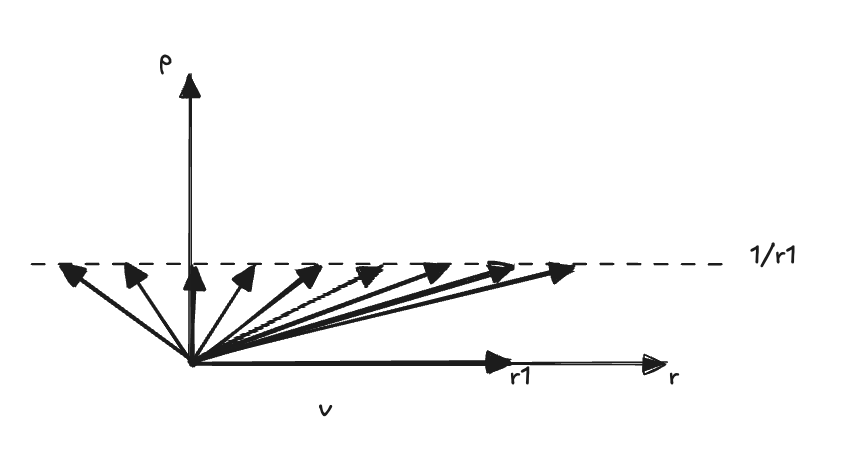
\includegraphics[scale=0.4]{ch2-12.png}
    \end{center}
\end{proof}
\cleardoublepage
\begin{proof}{\textbf{Exercise 13}}
    Let
    $$x_1 = \begin{pmatrix} r_1 \\p_1 \end{pmatrix}
    \quad x_2 = \begin{pmatrix} r_2 \\p_2 \end{pmatrix}$$
    Also, let $B$ be a $2\times 2$ matrix
    $$B = \begin{pmatrix} b_1 & b_2 \\ b_3 & b_4 \end{pmatrix}$$
    We know that 
    \begin{align*}
        A(x_1, x_2) = \det\begin{pmatrix}
            r_1 & r_2 \\ p_1 & p_2
        \end{pmatrix}
    \end{align*}
    So, we want to know the necessary and sufficient condition such that
    \begin{align*}
        \det(Bx_1, Bx_2) = \det(x_1, x_2)
    \end{align*}
    Hence, given that
    \begin{align*}
        Bx_1 = \begin{pmatrix}
            b1r_1 + b_2p_1\\ b_3r_1 + b_4p_1
        \end{pmatrix}
        \quad Bx_2 = \begin{pmatrix}
            b1r_2 + b_2p_2 \\ b_3r_2 + b_4p_2
        \end{pmatrix}
    \end{align*}
    We want that 
    \begin{align*}
        (b_1r_1 + b_2p_1)(b_3r_2 + b_4p_2) - (b_3r_1 + b_4p_1)(b_1r_2 + b_2p_2)
        &= r_1 p_2 - r_2 p_1\\
        (b_1r_1 + b_2p_1)b_3r_2 + (b_1r_1 + b_2p_1)b_4p_2 -\quad\\
        - (b_3r_1 + b_4p_1)b_1r_2 - (b_3r_1 + b_4p_1)b_2p_2
        &= r_1 p_2 - r_2 p_1\\
        b_1r_1b_3r_2 + b_2p_1b_3r_2 + b_1r_1b_4p_2 + b_2p_1b_4p_2 -\quad\\
        - b_3r_1b_1r_2 - b_4p_1b_1r_2 - b_3r_1b_2p_2 - b_4p_1b_2p_2
        &= r_1 p_2 - r_2 p_1\\
        b_2p_1b_3r_2 + b_1r_1b_4p_2 - b_4p_1b_1r_2 - b_3r_1b_2p_2
        &= r_1 p_2 - r_2 p_1\\
        r_1p_2(b_1b_4 - b_3b_2) - r_2p_1(b_1b_4 - b_3b_2)
        &= r_1 p_2 - r_2 p_1
    \end{align*}
    Then for this equality to be true we need that $b_1b_4 - b_3b_2 = 1$ i.e.
    \begin{align*}
        \det(B) = 1
    \end{align*}
\end{proof}
\cleardoublepage
\begin{proof}{\textbf{Exercise 14}}
\begin{itemize}
    \item [1.] We see that 
    \begin{align*}
        \bm{v}\times\bm{w}
        = (v_2w_3 - v_3w_2)\uvi + (v_3w_1 - v_1w_3)\uvj + (v_1w_2 - v_2w_1)\uvk
    \end{align*}
    Hence
    \begin{align*}
        \bm{u}\cdot(\bm{v}\times\bm{w})
        &= u_1(v_2w_3 - v_3w_2) + u_2(v_3w_1 - v_1w_3) + u_3(v_1w_2 - v_2w_1)\\
        &= u_1v_2w_3 - u_1v_3w_2 + u_2v_3w_1 - u_2v_1w_3 + u_3v_1w_2 - u_3v_2w_1\\
        &= (u_1v_2w_3 + u_2v_3w_1 + u_3v_1w_2) - (u_1v_3w_2 + u_2v_1w_3 + u_3v_2w_1)
    \end{align*}
    On the other hand, we see that
    \begin{align*}
        \det\begin{pmatrix}
            u_1 & v_1 & w_1\\
            u_2 & v_2 & w_2\\
            u_3 & v_3 & w_3
        \end{pmatrix}
        &= (u_1v_2w_3 + u_2v_3w_1 + u_3v_1w_2)\\
        &\quad- (u_3v_2w_1 + u_2v_1w_3 + u_1v_3w_2)
    \end{align*}
    Therefore
    \begin{align*}
        \det\begin{pmatrix}
            u_1 & v_1 & w_1\\
            u_2 & v_2 & w_2\\
            u_3 & v_3 & w_3
        \end{pmatrix} =
        \bm{u}\cdot(\bm{v}\times\bm{w})
    \end{align*}

    \item [2.] We know that $\bm{v}\times\bm{w}$ is a vector perpendicular
    to both vectors with a magnitude given by the area spanned by these vectors.
    So we can write that
    $$\bm{v}\times\bm{w} = A\bm{n}$$
    Where $A$ is the area spanned by these vectors.

    On the other hand, the dot product $\bm{u}\cdot(\bm{v}\times\bm{w})$ is
    the projection of $\bm{u}$ over $\bm{v}\times\bm{w}$ times the magnitude
    of the vector $\bm{v}\times\bm{w}$ i.e. the height of the parallelepiped
    times the area spanned by $\bm{v}$ and $\bm{w}$.

    Therefore $\bm{u}\cdot(\bm{v}\times\bm{w})$ represents the signed volume of
    the parallelepiped.

    \item [3.] Given that $\bm{u}\cdot(\bm{v} \times \bm{w})$ is the signed
    volume of the parallelepiped formed by these vectors then the products
    $\bm{v}\cdot(\bm{w} \times \bm{u})$ and $\bm{w}\cdot(\bm{u} \times \bm{v})$
    must be the same volume since the vectors involved are the same.

    Therefore must be that
    $\bm{u}\cdot(\bm{v} \times \bm{w}) = \bm{v}\cdot(\bm{w} \times \bm{u})
    = \bm{w}\cdot(\bm{u} \times \bm{v})$.
\cleardoublepage
    \item [4.]
    ($\Rightarrow$) Let $M$ be a $3 \times 3$ matrix with determinant 1
    and $f$ be a function $f:\R^3 \to \R^3$ such that $f$ takes $\bm{v}$ to
    $M\bm{v}$.
    
    Let us take the edges of the unit cube in $\R^3$ as $\bm{e_1} = (1, 0, 0)$,
    $\bm{e_2} = (0, 1, 0)$ and $\bm{e_3} = (0, 0, 1)$ then $f$ takes these unit
    vectors to $M\bm{e_1}, M\bm{e_2}$ and $M\bm{e_3}$ so the parallelepiped
    spanned by these vectors has a volume of
    $\det(M\bm{e_1}, M\bm{e_2}, M\bm{e_3})$ but we see that
    \begin{align*}
        \det(M\bm{e_1}, M\bm{e_2}, M\bm{e_3})
        = \det(M) = 1 
    \end{align*}
    Therefore the volume of the parallelepiped spanned by $M\bm{e_1}, M\bm{e_2}$
    and $M\bm{e_3}$ is 1 and so the unit cube is sent to a parallelepiped of
    signed volume 1.

    ($\Leftarrow$) Let $f$ be a function $f:\R^3 \to \R^3$ such that $f$ takes
    $\bm{v}$ to $M\bm{v}$ and $f$ takes the unit cube in the domain to 
    a parallelepiped of signed volume 1.

    Let us take the edges of the unit cube in $\R^3$ as $\bm{e_1} = (1, 0, 0)$,
    $\bm{e_2} = (0, 1, 0)$ and $\bm{e_3} = (0, 0, 1)$ then $f$ takes these unit
    vectors to $M\bm{e_1}, M\bm{e_2}$ and $M\bm{e_3}$. The parallelepiped
    spanned by these vectors has a volume of 1 by definition i.e.
    $\det(M\bm{e_1}, M\bm{e_2}, M\bm{e_3}) = 1$ but we see that
    \begin{align*}
        \det(M\bm{e_1}, M\bm{e_2}, M\bm{e_3})
        = \det(M) = 1 
    \end{align*}
    Therefore $M$ is a $3 \times 3$ matrix with determinant 1.
\end{itemize}
\end{proof}
\cleardoublepage
\begin{proof}{\textbf{Exercise 15}}

    ($\Rightarrow$) Let $M$ be a $n \times n$ matrix with determinant 1
    and $f$ be a function $f:\R^n \to \R^n$ such that $f$ takes $\bm{v}$ to
    $M\bm{v}$.
    
    Let us take the edges of the unit cube in $\R^n$ as
    $\bm{e_1} = (1, 0, 0, ..., 0)$, $\bm{e_2} = (0, 1, 0, ..., 0)$, ..., 
    $\bm{e_n} = (0, 0, 0, ..., 1)$ then $f$ takes these unit
    vectors to $M\bm{e_1}, M\bm{e_2}$, ..., $M\bm{e_n}$ so the parallelepiped
    spanned by these vectors has a volume of
    $\det(M\bm{e_1}, M\bm{e_2}, ..., M\bm{e_n})$ but we see that
    \begin{align*}
        \det(M\bm{e_1}, M\bm{e_2},..., M\bm{e_n})
        = \det(M) = 1 
    \end{align*}
    Therefore the volume of the parallelepiped spanned by $M\bm{e_1}, M\bm{e_2}$
    ..., $M\bm{e_n}$ is 1 and so the unit cube is sent to a parallelepiped of
    signed volume 1.

    ($\Leftarrow$) Let $f$ be a function $f:\R^n \to \R^n$ such that $f$ takes
    $\bm{v}$ to $M\bm{v}$ and $f$ takes the unit cube in the domain to 
    a parallelepiped of signed volume 1.

    Let us take the edges of the unit cube in $\R^n$ as
    $\bm{e_1} = (1, 0, 0, ..., 0)$, $\bm{e_2} = (0, 1, 0, ..., 0)$, ..., 
    $\bm{e_n} = (0, 0, 0, ..., 1)$ then $f$ takes these unit
    vectors to $M\bm{e_1}, M\bm{e_2}$, ..., $M\bm{e_n}$. The parallelepiped
    spanned by these vectors has a volume of 1 by definition i.e.
    $\det(M\bm{e_1}, M\bm{e_2}, ...,  M\bm{e_n}) = 1$ but we see that
    \begin{align*}
        \det(M\bm{e_1}, M\bm{e_2}, ..., M\bm{e_n})
        = \det(M) = 1 
    \end{align*}
    Therefore $M$ is a $n \times n$ matrix with determinant 1.
\end{proof}
\cleardoublepage
\begin{proof}{\textbf{Exercise 16}}
    Assume that
    \begin{align*}
        a_r\pdv{r} + a_p\pdv{p} = 0
    \end{align*}
    Then for all $f$ must be that
    \begin{align*}
        a_r\pdv{f}{r} + a_p\pdv{f}{p} = 0
    \end{align*}
    Suppose we take $f(r,p) = r$ then we have that $a_r = 0$.\\
    In the same way, if we take $f(r,p) = p$ we get that $a_p = 0$.

    Hence since $a_r\pdv{f}{r} + a_p\pdv{f}{p} = 0$
    needs to work for all $f$ must be that $a_r = a_p = 0$
    and therefore $\pdv{r}$ and $\pdv{p}$ are linearly independent.
\end{proof}
\begin{proof}{\textbf{Exercise 17}}
\begin{align*}
    \dv{t}~|_{t = 0} \int_{\bm{q}}^{\bm{q} + t\bm{v}} \alpha
    &= \dv{t}~|_{t = 0} \int_{(r_0, p_0)}^{(r_0, p_0) + t(v_1,v_2)} \alpha_1~dr + \alpha_2~dp\\
    &= \dv{t}~|_{t = 0} \left[\alpha_1 r+ \alpha_2 p
    \right]_{(r_0, p_0)}^{(r_0, p_0) + t(v_1,v_2)}\\
    &= \dv{t}~|_{t = 0} \left[(\alpha_1 (r_0 + tv_1)+ \alpha_2 (p_0 + tv_2))
    - (\alpha_1r_0 + \alpha_2 p_0)\right]\\
    &= \dv{t}~|_{t = 0} \left[\alpha_1 v_1 t + \alpha_2v_2 t\right]\\
    &= \alpha_1 v_1 + \alpha_2v_2
\end{align*}
\end{proof}
\cleardoublepage
\begin{proof}{\textbf{Exercise 18}}
    Let $F$ be an antisymmetric bilinear form then $F(\bm{v}, \bm{w})$ can be
    written as the following matrix operation
    \begin{align*}
        F(\bm{v}, \bm{w})
        &= \begin{pmatrix} v_1 & v_2 \end{pmatrix}
        \begin{pmatrix}
            f_{11} & f_{12}\\ f_{21} & f_{22}
        \end{pmatrix}
        \begin{pmatrix} w_1 \\ w_2 \end{pmatrix}\\
        &= w_1(v_1f_{11} + v_2f_{21}) + w_2(v_1f_{12} + v_2f_{22})
    \end{align*}
    But also since $F$ is an antisymmetric bilinear form we know that\\
    $F(\bm{v}, \bm{w}) = - F(\bm{w}, \bm{v})$ then must be that
    \begin{align*}
        w_1(v_1f_{11} + v_2f_{21}) + w_2(v_1f_{12} + v_2f_{22}) &=\\
        \quad -v_1(w_1f_{11} + w_2f_{21}) - v_2(w_1f_{12} &+ w_2f_{22})\\
        v_1w_1f_{11} + v_2w_1f_{21} + v_1w_2f_{12} + v_2w_2f_{22} &=\\
        \quad -v_1w_1f_{11} - v_1w_2f_{21} - v_2w_1f_{12} &-v_2w_2f_{22}\\
        2v_1w_1f_{11} + v_2w_1(f_{21} + f_{12}) + v_1w_2(f_{12} + f_{21})
        + 2v_2w_2f_{22} &= 0\\
        2v_1w_1f_{11} + (f_{12} + f_{21})(v_1w_2 + v_2w_1)
        + 2v_2w_2f_{22} &= 0
    \end{align*}
    But if $\bm{v}$ and $\bm{w}$ are not null then this equation can only be
    true if
    \begin{align*}
        f_{11} = 0 \qquad f_{12} + f_{21} = 0\qquad f_{22} = 0
    \end{align*}
    Or
    \begin{align*}
        f_{11} = 0 \qquad f_{21} = -f_{12}\qquad f_{22} = 0
    \end{align*}
    This implies that $F(\bm{v}, \bm{w})$ must be
    \begin{align*}
        F(\bm{v}, \bm{w})
        &= \begin{pmatrix} v_1 & v_2 \end{pmatrix}
        \begin{pmatrix}
            0 & f_{12}\\ -f_{12} & 0
        \end{pmatrix}
        \begin{pmatrix} w_1 \\ w_2 \end{pmatrix}
    \end{align*}
    Therefore $F$ has a correspondence to a antisymmetric $2\times2$ matrix.
\end{proof}
\begin{proof}{\textbf{Exercise 19}}
    Let $\alpha, \beta$ be covectors and $\bm{v},\bm{w}$ be vectors then the
    wedge product of $\alpha$ and $\beta$ is given by
    \begin{align*}
        (\alpha \wedge\beta)(\bm{v}, \bm{w})
        = (\alpha\bm{v})(\beta\bm{w}) - (\alpha\bm{w})(\beta\bm{v}) 
    \end{align*}
    On the other hand, we see that
    \begin{align*}
        -(\beta \wedge\alpha)(\bm{v}, \bm{w})
        &= -((\beta\bm{v})(\alpha\bm{w}) - (\beta\bm{w})(\alpha\bm{v}))\\
        &= (\beta\bm{w})(\alpha\bm{v}) -(\beta\bm{v})(\alpha\bm{w})\\
        &= (\alpha\bm{v})(\beta\bm{w}) -(\alpha\bm{w})(\beta\bm{v})
    \end{align*}
    Where we used commutativity of scalars in the last step, so
    $$(\alpha \wedge\beta)(\bm{v}, \bm{w}) = -(\beta \wedge\alpha)(\bm{v}, \bm{w})$$
    Therefore the wedge product is itself antisymmetric.
\end{proof}
\cleardoublepage
\begin{proof}{\textbf{Exercise 20}}
    Let $F$ be an antisymmetric bilinear form then $F(\bm{v}, \bm{w})$ can
    be written as
    \begin{align*}
        F(\bm{v}, \bm{w}) &= \begin{pmatrix} v_1 & v_2 \end{pmatrix}
        \begin{pmatrix}
            0 & f_{12}\\ -f_{12} & 0
        \end{pmatrix}
        \begin{pmatrix} w_1 \\ w_2 \end{pmatrix}\\
        &= f_{12}w_2v_1 - f_{12}w_1v_2
    \end{align*}
    If we take two covectors
    \begin{align*}
        \alpha = (0\quad f_{12}) \quad \text{ and } \quad \beta = (-1\quad 0)
    \end{align*}
    Then the wedge product of this covectors become
    \begin{align*}
        (\alpha \wedge\beta)(\bm{v}, \bm{w})
        &= (\alpha\bm{v})(\beta\bm{w}) - (\alpha\bm{w})(\beta\bm{v})\\
        &= (0\quad f_{12})\begin{pmatrix} v_1 \\ v_2 \end{pmatrix}
        (-1\quad 0)\begin{pmatrix} w_1 \\ w_2 \end{pmatrix} -\\
        &\quad - (0\quad f_{12})\begin{pmatrix} w_1 \\ w_2 \end{pmatrix}
        (-1\quad 0)\begin{pmatrix} v_1 \\ v_2 \end{pmatrix}\\
        &= (f_{12}v_2)(-w_1) - (f_{12}w_2)(-v_1)\\
        &= f_{12}w_2v_1 - f_{12}w_1v_2
    \end{align*}
    Therefore we see that $F(\bm{v}, \bm{w}) = (\alpha \wedge\beta)(\bm{v}, \bm{w})$
    for $\alpha, \beta$ defined as mentioned.
\end{proof}
\cleardoublepage
\begin{proof}{\textbf{Exercise 21}}
    Let $F$ be an antisymmetric bilinear form on $\R^3$ then $F(\bm{v}, \bm{w})$
    can be written as
    \begin{align*}
        F(\bm{v}, \bm{w}) &= \begin{pmatrix} v_1 & v_2 & v_3 \end{pmatrix}
        \begin{pmatrix}
            0 & f_{12} & f_{13}\\
            -f_{12} & 0 & f_{23}\\
            -f_{13} & -f_{23} & 0\\
        \end{pmatrix}
        \begin{pmatrix} w_1 \\ w_2 \\ w_3\end{pmatrix}\\
        &= w_1(-f_{12}v_2 -f_{13}v_3) + w_2(f_{12}v_1 - f_{23}v_3)
        + w_3(f_{13}v_1 + f_{23}v_2)\\
        &= f_{12}(w_2v_1 - w_1v_2) + f_{13}(w_3v_1 - w_1v_3)
        + f_{23}(w_3v_2 - w_2v_3)
    \end{align*}
    If we take two covectors
    \begin{align*}
        \alpha &= (0 \quad f_{13}\quad f_{23})\\
        \beta &= (-1\quad 0\quad f_{23}/f_{12})
    \end{align*}
    Then the wedge product of this covectors become
    \begin{align*}
        (\alpha \wedge\beta)(\bm{v}, \bm{w})
        &= (\alpha\bm{v})(\beta\bm{w}) - (\alpha\bm{w})(\beta\bm{v})\\
        &= (0\quad f_{12}\quad f_{13})
        \begin{pmatrix} v_1 \\ v_2 \\ v_3\end{pmatrix}
        (-1\quad 0\quad f_{23}/f_{12})
        \begin{pmatrix} w_1 \\ w_2 \\ w_3\end{pmatrix} -\\
        &\quad - (0\quad f_{12}\quad f_{13})
        \begin{pmatrix} w_1 \\ w_2 \\ w_3\end{pmatrix}
        (-1\quad 0\quad f_{23}/f_{12})
        \begin{pmatrix} v_1 \\ v_2 \\ v_3\end{pmatrix}\\
        &= (f_{12}v_2 + f_{13}v_3)\left(-w_1 + \frac{f_{23}}{f_{12}}w_3\right)
        - (f_{12}w_2 + f_{13}w_3)\left(-v_1 + \frac{f_{23}}{f_{12}}v_3\right)\\
        &= -f_{12}v_2w_1 - f_{13}v_3w_1 + f_{23}v_2w_3
        + f_{13}\frac{f_{23}}{f_{12}}v_3w_3\\
        &\quad + f_{12}v_1w_2 + f_{13}v_1w_3 - f_{23}v_3w_2
        - f_{13}\frac{f_{23}}{f_{12}}v_3w_3\\
        &= f_{12}(v_1w_2 -v_2w_1) + f_{13}(v_1w_3- v_3w_1)
        + f_{23}(v_2w_3 - v_3w_2)
    \end{align*}
    Therefore we see that $F(\bm{v}, \bm{w}) = (\alpha \wedge\beta)(\bm{v}, \bm{w})$
    for $\alpha, \beta$ defined as mentioned.
\end{proof}
\cleardoublepage
\begin{proof}{\textbf{Exercise 22}}
    Let us consider a $4\times4$ antisymmetric matrix
    \begin{align*}
        \begin{pmatrix}
            0 & a & b & c\\
            -a & 0 & d & e\\
            -b & -d & 0 & f\\
            -c & -e & -f & 0
        \end{pmatrix}
    \end{align*}
    This matrix will be of rank 4 if the only solution to the following
    system of equations is $\alpha = \beta = \delta = \epsilon = 0$
    \begin{align*}
        \alpha(0, -a, -b, -c) + \beta(a, 0, -d, -e) + \delta(b, d, 0, -f)
        + \epsilon(c, e, f, 0) = (0, 0, 0, 0)
    \end{align*}
    If we let $a = b = c = d = e = f = 1$ we get a matrix
    \begin{align*}
        A = 
        \begin{pmatrix}
            0 & 1 & 1 & 1\\
            -1 & 0 & 1 & 1\\
            -1 & -1 & 0 & 1\\
            -1 & -1 & -1 & 0
        \end{pmatrix}
    \end{align*}
    and hence the followeing system of equations
    \begin{align*}
        \beta + \delta + \epsilon &= 0\\
        -\alpha + \delta + \epsilon &= 0\\
        -\alpha - \beta + \epsilon &= 0\\
        -\alpha - \beta - \delta &= 0
    \end{align*}
    Which has no solutions other than $\alpha = \beta = \delta = \epsilon = 0$.
    Therefore $A$ is a rank 4 matrix and hence an invertible matrix which
    shows it cannot be written as a wedge product of two covectors.

    Let now $F$ be an antisymmetric bilinear form on $\R^4$ then
    $F(\bm{v},\bm{w})$ can be written as
    \begin{align*}
        F(\bm{v}, \bm{w}) &= \begin{pmatrix} v_1 & v_2 & v_3 & v_4 \end{pmatrix}
        \begin{pmatrix}
            0 & a & b & c\\
            -a & 0 & d & e\\
            -b & -d & 0 & f\\
            -c & -e & -f & 0\\
        \end{pmatrix}
        \begin{pmatrix} w_1 \\ w_2 \\ w_3\\ w_4\end{pmatrix}\\
        &= w_1(-av_2 -bv_3 -cv_4) + w_2(av_1 -dv_3 -ev_4) + w_3(bv_1 + dv_2 -fv_4)\\
        &\quad + w_4(cv_1 + ev_2 + fv_3)\\
        &= a(w_2v_1-w_1v_2) + b(w_3v_1-w_1v_3) + c(w_4v_1-w_1v_4) + d(w_3v_2-w_2v_3)\\
        &\quad + e(w_4v_2-w_2v_4) + f(w_4v_3-w_3v_4)
    \end{align*}
    If we take two covectors
    \begin{align*}
        \alpha = (1\quad 0)\\
        \beta = (0\quad 1)
    \end{align*}
    Then we see that 
    \begin{align*}
        (\alpha\wedge\beta)\begin{pmatrix}
            \begin{pmatrix} v_1\\ v_2 \end{pmatrix},
            \begin{pmatrix} w_1\\ w_2 \end{pmatrix}
        \end{pmatrix}
        &= (1\quad 0)\begin{pmatrix} v_1\\ v_2 \end{pmatrix}
        (0\quad 1)\begin{pmatrix} w_1\\ w_2 \end{pmatrix} -
        (1\quad 0)\begin{pmatrix} w_1\\ w_2 \end{pmatrix}
        (0\quad 1)\begin{pmatrix} v_1\\ v_2 \end{pmatrix}\\
        &= w_2v_1 - w_1v_2
    \end{align*}
    Then we can write that
    \begin{align*}
        F(\bm{v}, \bm{w}) &= a\bigg[(\alpha\wedge\beta)\begin{pmatrix}
            \begin{pmatrix} v_1\\ v_2 \end{pmatrix},
            \begin{pmatrix} w_1\\ w_2 \end{pmatrix}
        \end{pmatrix}\bigg] + b\bigg[(\alpha\wedge\beta)\begin{pmatrix}
            \begin{pmatrix} v_1\\ v_3 \end{pmatrix},
            \begin{pmatrix} w_1\\ w_3 \end{pmatrix}
        \end{pmatrix}\bigg]\\
        &\quad + c\bigg[(\alpha\wedge\beta)\begin{pmatrix}
            \begin{pmatrix} v_1\\ v_4 \end{pmatrix},
            \begin{pmatrix} w_1\\ w_4 \end{pmatrix}
        \end{pmatrix}\bigg] + d\bigg[(\alpha\wedge\beta)\begin{pmatrix}
            \begin{pmatrix} v_2\\ v_3 \end{pmatrix},
            \begin{pmatrix} w_2\\ w_3 \end{pmatrix}
        \end{pmatrix}\bigg]\\
        &\quad + e\bigg[(\alpha\wedge\beta)\begin{pmatrix}
            \begin{pmatrix} v_2\\ v_4 \end{pmatrix},
            \begin{pmatrix} w_2\\ w_4 \end{pmatrix}
        \end{pmatrix}\bigg] + f\bigg[(\alpha\wedge\beta)\begin{pmatrix}
            \begin{pmatrix} v_3\\ v_4 \end{pmatrix},
            \begin{pmatrix} w_3\\ w_4 \end{pmatrix}
        \end{pmatrix}\bigg]
    \end{align*}
    Therefore we can write every antisymmetric bilinear form on $\R^4$ as
    a finite linear combination of wedge products of covectors.
\end{proof}
\cleardoublepage
\begin{proof}{\textbf{Exercise 23}}
    Let us define
    \begin{align*}
        dr_1 &= (1 ~ 0 ~ 0 ~ 0 ~ 0 ~ 0)
        \qquad dp_1 = (0 ~ 0 ~ 0 ~ 1 ~ 0 ~ 0)\\
        dr_2 &= (0 ~ 1 ~ 0 ~ 0 ~ 0 ~ 0)
        \qquad dp_2 = (0 ~ 0 ~ 0 ~ 0 ~ 1 ~ 0)\\
        dr_3 &= (0 ~ 0 ~ 1 ~ 0 ~ 0 ~ 0)
        \qquad dp_3 = (0 ~ 0 ~ 0 ~ 0 ~ 0 ~ 1)
    \end{align*}
    Also, let us take $\bm{v}$ and $\bm{w}$ in $\R^6$ with the following
    components
    \begin{align*}
        \bm{v} &= (v_{rx}~v_{ry}~v_{rz}~v_{px}~v_{py}~v_{pz})\\
        \bm{w} &= (w_{rx} ~ w_{ry} ~ w_{rz} ~ w_{px} ~ w_{py} ~ w_{pz})
    \end{align*}
    Then $(dr_1 \wedge dp_1)(\bm{v}, \bm{w})$ is given by
    \begin{align*}
        (dr_1 \wedge dp_1)(\bm{v}, \bm{w})
        &= (dr_1\bm{v})(dp_1\bm{w}) - (dr_1\bm{w})(dp_1\bm{v})\\
        &= v_{rx}w_{px} - w_{rx}v_{px}
    \end{align*}
    Hence in the same way we have that
    \begin{align*}
        (dr_2 \wedge dp_2)(\bm{v}, \bm{w}) &= v_{ry}w_{py} - w_{ry}v_{py}\\
        (dr_3 \wedge dp_3)(\bm{v}, \bm{w}) &= v_{rz}w_{pz} - w_{rz}v_{pz}
    \end{align*}
    Then
    \begin{align*}
        &(dr_1 \wedge dp_1 + dr_2 \wedge dp_2 + dr_3 \wedge dp_3)
        (\bm{v}, \bm{w}) = \\
        &\quad = v_{rx}w_{px} - w_{rx}v_{px}
        + v_{ry}w_{py} - w_{ry}v_{py}
        + v_{rz}w_{pz} - w_{rz}v_{pz}\\
        &\quad = (-v_{px} ~ -v_{py} ~ -v_{pz} ~ v_{rx} ~ v_{ry} ~ v_{rz})
        \begin{pmatrix}
            w_{rx} \\ w_{ry} \\ w_{rz} \\ w_{px} \\ w_{py} \\ w_{pz}
        \end{pmatrix}
    \end{align*}
    Therefore the antisymmetric $6\times 6$ matrix corresponding to the
    bilinear form mentioned above is 
    \begin{align*}
        \begin{pmatrix}
            0  &  0  &  0  &  1  &  0  &  0 \\
            0  &  0  &  0  &  0  &  1  &  0 \\
            0  &  0  &  0  &  0  &  0  &  1 \\
           -1  &  0  &  0  &  0  &  0  &  0 \\
            0  & -1  &  0  &  0  &  0  &  0 \\
            0  &  0  & -1  &  0  &  0  &  0 \\
        \end{pmatrix}
    \end{align*}
\end{proof}
\cleardoublepage
\begin{proof}{\textbf{Exercise 24}}
    Let $F$ be an antisymmetric bilinear form on $\R^n$ then
    $F(\bm{v}, \bm{w})$ can be written as the following matrix operation
    \begin{align*}
        F(\bm{v}, \bm{w})
        &= \begin{pmatrix} v_1 & v_2 & ... & v_n\end{pmatrix}
        \begin{pmatrix}
            f_{11} & f_{12} & ... & f_{1n}\\
            f_{21} & f_{22} & ... & f_{2n}\\
            \vdots & \vdots & ... & \vdots\\
            f_{n1} & f_{n2} & ... & f_{nn}\\
        \end{pmatrix}
        \begin{pmatrix} w_1 \\ w_2 \\ \vdots \\ w_n\end{pmatrix}\\
        &= w_1(v_1 f_{11} + v_2 f_{21} + ... + v_n f_{n1}) +
        w_2(v_1 f_{12} + v_2 f_{22} + ... + v_n f_{n2}) +\\
        \quad& + ... + w_n(v_1 f_{1n} + v_2 f_{2n} + ... + v_n f_{nn})
    \end{align*}
    But also since $F$ is an antisymmetric bilinear form we know that\\
    $F(\bm{v}, \bm{w}) = - F(\bm{w}, \bm{v})$ then must be that
    \begin{align*}
        &w_1(v_1 f_{11} + v_2 f_{21} + ... + v_n f_{n1})
        + w_2(v_1 f_{12} + v_2 f_{22} + ... + v_n f_{n2}) + ...\\
        &+ w_n(v_1 f_{1n} + v_2 f_{2n} + ... + v_n f_{nn})
        = -v_1(w_1 f_{11} + w_2 f_{21} + ... + w_n f_{n1})\\
        &-v_2(w_1 f_{12} + w_2 f_{22} + ... + w_n f_{n2})
        - ... - v_n(w_1 f_{1n} + w_2 f_{2n} + ... + w_n f_{nn})
    \end{align*}
    Hence
    \begin{align*}
        &2w_1v_1 f_{11} + w_1v_2(f_{21} + f_{12}) + ... + w_1v_n(f_{n1} + f_{1n})\\
        &+ w_2v_1(f_{12} + f_{21}) + 2w_2v_2f_{22} + ... + w_2v_n(f_{n2} + f_{2n})\\
        &+ ... + w_nv_1(f_{1n} + f_{n1}) + w_nv_2(f_{2n} + f_{n2})
        + ... + 2w_nv_nf_{nn}\\
        &= 0
    \end{align*}
    But if $\bm{v}$ and $\bm{w}$ are not null then this equation can only be
    true if
    \begin{align*}
        f_{ij} = \begin{cases}
            0 &\text{ when } i = j\\
            -f_{ji} &\text{ when } i \neq j
        \end{cases}
    \end{align*}
    This implies that $F(\bm{v}, \bm{w})$ must be
    \begin{align*}
        F(\bm{v}, \bm{w})
        &= \begin{pmatrix} v_1 & v_2 & ... & v_n\end{pmatrix}
        \begin{pmatrix}
            0 & f_{12} & ... & f_{1n}\\
            -f_{12} & 0 & ... & f_{2n}\\
            \vdots & \vdots & ... & \vdots\\
            -f_{1n} & -f_{2n} & ... & 0\\
        \end{pmatrix}
        \begin{pmatrix} w_1 \\ w_2 \\ \vdots \\ w_n\end{pmatrix}
    \end{align*}
    Therefore $F$ has a correspondence to a antisymmetric $n\times n$ matrix.
\end{proof}
\cleardoublepage
\begin{proof}{\textbf{Exercise 25}}
    Let $\alpha$ be a covector and $\beta$ an antisymmetric bilinear form on
    $\R^n$ then $\alpha \wedge \beta$ is given by
    \begin{align*}
        (\alpha\wedge\beta)(\bm{u}, \bm{v}, \bm{w})
        = \alpha(\bm{u})\beta(\bm{v}, \bm{w}) + \alpha(\bm{v})\beta(\bm{w}, \bm{u})
        + \alpha(\bm{w})\beta(\bm{u}, \bm{v})
    \end{align*}
    Also, we have that
    \begin{align*}
        -(\alpha\wedge\beta)(\bm{v}, \bm{u}, \bm{w})
        &= -(\alpha(\bm{v})\beta(\bm{u}, \bm{w}) + \alpha(\bm{u})\beta(\bm{w}, \bm{v})
        + \alpha(\bm{w})\beta(\bm{v}, \bm{u}))\\
        &= \alpha(\bm{v})(-\beta(\bm{u}, \bm{w})) + \alpha(\bm{u})(-\beta(\bm{w}, \bm{v}))
        + \alpha(\bm{w})(-\beta(\bm{v}, \bm{u}))\\
        &= \alpha(\bm{v})\beta(\bm{w}, \bm{u}) + \alpha(\bm{u})\beta(\bm{v}, \bm{w})
        + \alpha(\bm{w})\beta(\bm{u}, \bm{v})\\
        &= (\alpha\wedge\beta)(\bm{u}, \bm{v}, \bm{w})
    \end{align*}
    Where we used that $\beta$ is an antisymmetric bilinear form and hence
    $\beta(\bm{u},\bm{v}) = -\beta(\bm{v},\bm{u})$.\\
    Finally, we see that
    \begin{align*}
        (\alpha\wedge\beta)(\bm{v}, \bm{w}, \bm{u})
        &= \alpha(\bm{v})\beta(\bm{w}, \bm{u}) + \alpha(\bm{w})\beta(\bm{u}, \bm{v})
        + \alpha(\bm{u})\beta(\bm{v}, \bm{w})\\
        &= \alpha(\bm{u})\beta(\bm{v}, \bm{w}) + \alpha(\bm{v})\beta(\bm{w}, \bm{u})
        + \alpha(\bm{w})\beta(\bm{u}, \bm{v})\\
        &= (\alpha\wedge\beta)(\bm{u}, \bm{v}, \bm{w})
    \end{align*}
    Where we only re-ordered the terms. Therefore
    $$(\alpha\wedge\beta)(\bm{u}, \bm{v}, \bm{w})
    = -(\alpha\wedge\beta)(\bm{v}, \bm{u}, \bm{w})
    = (\alpha\wedge\beta)(\bm{v}, \bm{w}, \bm{u})$$
    So $\alpha\wedge\beta$ is alternating.
\end{proof}
\cleardoublepage
\begin{proof}{\textbf{Exercise 26}}
    By definition $\pdv{\theta}$ is
    $\pdv{\theta}(\rho\cos\theta, \rho\sin\theta)^T$ hence
    \begin{align*}
        \pdv{\theta} = \begin{pmatrix}
            \rho~\pdv{\theta}(\cos\theta)\\
            \rho~\pdv{\theta}(\sin\theta)
        \end{pmatrix}
        = \begin{pmatrix}
            -\rho\sin\theta\\
            \rho\cos\theta
        \end{pmatrix}
        = \begin{pmatrix}
            -p \\ r
        \end{pmatrix}
    \end{align*}
    If we recall that
    \begin{align*}
        \pdv{r} = \begin{pmatrix}1\\0\end{pmatrix} \qquad
        \pdv{p} = \begin{pmatrix}0\\1\end{pmatrix}
    \end{align*}
    We can write that
    \begin{align*}
        \pdv{\theta} = -p\pdv{r} + r\pdv{p}
    \end{align*}
    Now, let us define $\pdv{\rho}$ as $\pdv{\rho}(\rho\cos\theta, \rho\sin\theta)^T$
    then we have that
    \begin{align*}
        \pdv{\rho} = \begin{pmatrix}
            \cos\theta\\
            \sin\theta
        \end{pmatrix}
        = \begin{pmatrix}r/\rho\\ p/\rho\end{pmatrix}
        = \begin{pmatrix}
            \frac{r}{\sqrt{r^2 + p^2}}\\ \frac{p}{\sqrt{r^2 + p^2}}
        \end{pmatrix}
        = \frac{1}{\sqrt{r^2 + p^2}}\begin{pmatrix}
            r\pdv{r} + p\pdv{p}
        \end{pmatrix}
    \end{align*}
    Where we used that $\rho = \sqrt{r^2 + p^2}$.

    Finally, let $f:\R^2 \to \R$ be a differentiable function then
    $\pdv{f}{\theta}$ is given by
    \begin{align*}
        \pdv{f}{\theta} &= -p\pdv{f}{r} + r\pdv{f}{p}\\
        &= -\rho\sin\theta\pdv{f}{r} + \rho\cos\theta\pdv{f}{p}\\
        &= \rho(\cos\theta\pdv{f}{p} - \sin\theta\pdv{f}{r})
    \end{align*}
    On the other hand, $\pdv{f}{\rho}$ is 
    \begin{align*}
        \pdv{f}{\rho}
        &= \frac{1}{\sqrt{r^2 + p^2}}\bigg(r\pdv{f}{r} + p\pdv{f}{p}\bigg)\\
        &= \frac{1}{\rho}\bigg(\rho\cos\theta\pdv{f}{r}
        + \rho\sin\theta\pdv{f}{p}\bigg)\\
        &= \cos\theta\pdv{f}{r} + \sin\theta\pdv{f}{p}
    \end{align*}
\end{proof}
\cleardoublepage
\begin{proof}{\textbf{Exercise 27}}
    Let $f: \R^n \to \R$ then the gradient one-form of $f$ i.e. $df$ is
    by definition
    \begin{align*}
        df = \begin{pmatrix}
            \pdv{f}{x_1}, \pdv{f}{x_2}, ..., \pdv{f}{x_n} 
        \end{pmatrix}
    \end{align*}
    But also $J_f$ by definition is the matrix of all possible first partial
    derivatives with one column for each independent (domain) variable and one
    row for each dependent (range) variable. Therefore
    \begin{align*}
        J_f = \begin{pmatrix}
            \pdv{f}{x_1}, \pdv{f}{x_2}, ..., \pdv{f}{x_n} 
        \end{pmatrix} = df
    \end{align*}
    If we let $n = 1$ then $f:\R \to \R$ which implies that
    \begin{align*}
        J_f = \begin{pmatrix}
            \pdv{f}{x_1} 
        \end{pmatrix} = f'
    \end{align*}
\end{proof}
\begin{proof}{\textbf{Exercise 29}}
    Let $f:\R^3 \to \R^3$ then $f$ can be written as 
    \begin{align*}
        \begin{pmatrix} x \\ y \\ z \end{pmatrix}
        \to \begin{pmatrix} f_x(x,y,z)\\ f_y(x,y,z)\\ f_z(x,y,z) \end{pmatrix}
    \end{align*}
    So the Jacobian, $J_f$ is given by
    \begin{align*}
        J_f = \begin{pmatrix}
            \pdv{f_x}{x} & \pdv{f_x}{y} & \pdv{f_x}{z}\\[1ex]
            \pdv{f_y}{x} & \pdv{f_y}{y} & \pdv{f_y}{z}\\[1ex]
            \pdv{f_z}{x} & \pdv{f_z}{y} & \pdv{f_z}{z}
        \end{pmatrix}
    \end{align*}
    Hence
    $$\tr J_f = \pdv{f_x}{x} + \pdv{f_y}{y} +\pdv{f_z}{z}$$
    On the other hand if we treat $f$ as a vector field
    $f = f_x \uvi + f_y \uvj + f_z \uvk$ then we can compute its divergence
    as
    \begin{align*}
        \div{f} = \left(\pdv{x}, \pdv{y}, \pdv{z}\right)\cdot (f_x, f_y, f_z)
        = \pdv{f_x}{x} + \pdv{f_y}{y} +\pdv{f_z}{z}
    \end{align*}
    Therefore $\div{f} = \tr J_f$
\end{proof}

\cleardoublepage
\begin{proof}{\textbf{Exercise 30}}
Let $\Psi: \R^2 \to \R^2$ be the function that parametrizes the plane by polar
coordinates defined as 
\begin{align*}
    \begin{pmatrix} \theta\\ \rho \end{pmatrix}
    \to \begin{pmatrix} \rho\cos\theta\\ \rho\sin\theta \end{pmatrix}
\end{align*}
Then
\begin{align*}
    \pdv{\Psi}{\theta} = \begin{pmatrix} -\rho\sin\theta\\ \rho\cos\theta
    \end{pmatrix}\qquad
    \pdv{\Psi}{\rho} = \begin{pmatrix} \cos\theta\\ \sin\theta\end{pmatrix}
\end{align*}
So the Jacobian of $\Psi$ is
\begin{align*}
    J_{\Psi}(\theta, \rho) =
    \begin{pmatrix}
        -\rho\sin\theta & \cos\theta\\
        \rho\cos\theta & \sin\theta
    \end{pmatrix}
\end{align*}
Now let $f:\R^2 \to \R$ be an arbitrary function then via the chain rule
we have that
\begin{align*}
    J_{f \circ \Psi}(\theta, \rho) 
    &= J_{f}(\Psi(\theta, \rho))J_{\Psi}(\theta, \rho)\\
    \begin{pmatrix} \pdv{f\circ\Psi}{\theta} & \pdv{f\circ\Psi}{\rho}
    \end{pmatrix}
    &=
    \begin{pmatrix} \pdv{f}{r} & \pdv{f}{p}
    \end{pmatrix}\cdot
    \begin{pmatrix}
        -\rho\sin\theta & \cos\theta\\
        \rho\cos\theta & \sin\theta
    \end{pmatrix}
\end{align*}
Then we have that
\begin{align*}
    \pdv{f\circ\Psi}{\theta}
    &= -\rho\sin\theta\pdv{f}{r} + \rho\cos\theta\pdv{f}{p}
    = -p\pdv{f}{r} + r\pdv{f}{p}\\
    \pdv{f\circ\Psi}{\rho}
    &= \cos\theta\pdv{f}{r} + \sin\theta\pdv{f}{p}
    = \frac{1}{\sqrt{r^2 + p^2}} \bigg(r\pdv{f}{r} + p\pdv{f}{p}\bigg)
\end{align*}
Where we used that $(\cos\theta,~\sin\theta)^T = (r/\rho,~p/\rho)^T$.
Since in the calculations we used an arbitrary function $f$ then we can write
that
\begin{align*}
    \pdv{}{\theta} &= -p\pdv{}{r} + r\pdv{}{p}\\
    \pdv{}{\rho}
    &= \frac{1}{\sqrt{r^2 + p^2}} \bigg(r\pdv{}{r} + p\pdv{}{p}\bigg)
\end{align*}
Which is the same result we got in Exercise 26.
\end{proof}

\cleardoublepage
\begin{proof}{\textbf{Exercise 31}}
Let
$$\omega = dp_1 \wedge dr_1 + dp_2 \wedge dr_2 + ... + dp_n \wedge dr_n$$
We know that $(dp_1 \wedge dr_1)(\bm{v}, \bm{w})$ is the signed area
of the parallelogram spanned by the projection of the vectors $\bm{v}$ and
$\bm{w}$ over the $r_1$-$p_1$ plane.

Therefore $\omega(\bm{v}, \bm{w})$ is the sum of the signed areas of the
parallelograms spanned by the projections of the vectors $\bm{v}$ and
$\bm{w}$ over the $r_i$-$p_i$ planes.
\end{proof}

\cleardoublepage
\begin{proof}{\textbf{Exercise 32}}
    Let 
    $$T^*S^2 = \{(\bm{r},\bm{p}) \in \R^3 \times (\R^3)^* :
    |\bm{r}|=1 \text{ and } \bm{pr} = 0\}$$
    Hence elements in $T^*S^2$ needs to satisfy
    \begin{align*}
        r_1^2 + r_2^2 + r_3^2 = 1 \qquad
        p_1r_1 + p_2r_2 + p_3r_3 = 0
    \end{align*}
    So we define a function $F:\R^6 \to \R^2$ such that for any $\bm{c} \in \R^6$
    we have that $F(\bm{c}) = 0$ as
    \begin{align*}
        F\begin{pmatrix}\bm{r}\\\bm{p}\end{pmatrix} = \begin{pmatrix}
            r_1^2 + r_2^2 + r_3^2 - 1\\
            p_1r_1 + p_2r_2 + p_3r_3
        \end{pmatrix}
    \end{align*}
    Then the Jacobian of this function is 
    \begin{align*}
        J_F(\bm{r}, \bm{p}) = \begin{pmatrix}
            2r_1 & 2r_2 & 2r_3 & 0   & 0   & 0 \\
            p_1  & p_2  & p_3  & r_1 & r_2 & r_3
        \end{pmatrix}
    \end{align*}
    Since not all $r_i$ can be $0$ at the same time since we are considering
    a sphere then both rows are linearly independent so the rank of this
    Jacobian is 2 (full rank) and hence it is onto.\\
    Then the Implicit function theorem guarantees that in some neighbourhood of
    $\bm{c}$ in which $F = 0$ the equation for $F$ implicitly expresses
    one of the variables in terms of the others.\\
    Suppose $r_1 \neq 0$ then we can write explicitly the equations as follows
    \begin{align*}
        r_1 = \sqrt{1 -r_2^2 - r_3^2}\\
        p_1 = \frac{-p_2r_2 - p_3r_3}{r_1}
    \end{align*}
    The same can be done assuming that $r_2 \neq 0$ or $r_3 \neq 0$.\\
    Therefore, we can parametrize the function $F$ by a function $g$ as follows
    \begin{align*}
        g:\begin{pmatrix}r_2 \\ r_3 \\ p_2 \\ p_3\end{pmatrix}
        \to
        \begin{pmatrix}
            \sqrt{1 -r_2^2 - r_3^2}\\[6pt] r_2\\[6pt] r_3\\[6pt]
            \frac{-p_2r_2 - p_3r_3}{\sqrt{1 -r_2^2 - r_3^2}}\\[6pt]
            p_2\\[6pt] p_3\\[6pt]
        \end{pmatrix}
    \end{align*}
    Hence $T^*S^2$ can be parametrized by four real parameters.
\end{proof}

\cleardoublepage
\begin{proof}{\textbf{Exercise 33}}
Let $f$ be the distance function in Cartesian coordinates i.e.
$$f\begin{pmatrix}r \\ p\end{pmatrix} = \sqrt{r^2 + p^2}$$
Then $\Gamma^* f = f \circ \Gamma$ is given by
\begin{align*}
    f \circ \Gamma\begin{pmatrix}\rho \\ \theta \end{pmatrix}
    &= f\begin{pmatrix}
        \rho\cos\theta \\  \rho\sin\theta
    \end{pmatrix}\\
    &= \sqrt{(\rho\cos\theta)^2 + (\rho\sin\theta)^2}\\
    &= \sqrt{\rho^2(\cos^2\theta + \sin^2\theta)}\\
    &= \rho
\end{align*}
Therefore $f\circ \Gamma$ is the function
\begin{align*}
    \begin{pmatrix}\rho \\ \theta \end{pmatrix} \to \rho
\end{align*}
\end{proof}
\begin{proof}{\textbf{Exercise 34}} We know $p = \rho\sin\theta$ then
\begin{align*}
    dp &= d(\rho \sin\theta)\\
    &= \bigg(\pdv{\rho}\rho \sin\theta~~\pdv{\theta}\rho \sin\theta\bigg)\\
    &= \bigg(\sin\theta~~\rho \cos\theta\bigg)\\
    &= \sin\theta~d\rho + \rho \cos\theta~d\theta
\end{align*}
\end{proof}
\begin{proof}{\textbf{Exercise 35}}
We compute $dr\cdot J_\Gamma$ as follows
\begin{align*}
    dr\cdot J_\Gamma &= \begin{pmatrix} 1 & 0 \end{pmatrix}
    \begin{pmatrix}
        \cos\theta & -\rho\sin\theta\\
        \sin\theta & \rho\cos\theta
    \end{pmatrix}\\
    &= \begin{pmatrix}
        \cos\theta & -\rho\sin\theta
    \end{pmatrix}\\
    &= \cos\theta d\rho -\rho\sin\theta d\theta
\end{align*}
\end{proof}

\cleardoublepage
\begin{proof}{\textbf{Exercise 36}}
Let us define new coordinates by
\begin{align*}
    \begin{pmatrix} r \\ p \end{pmatrix}
    = M  \begin{pmatrix} x \\ y \end{pmatrix}
\end{align*}
Where $M$ is a constant $2\times 2$ invertible matrix
\begin{itemize}
\item [1.] From the definition we know that $r$ and $p$ can be written as
\begin{align*}
    r = ax + by \quad
    p = cx + dy
\end{align*}
Where $a, b, c $ and $d$ are the coefficients of $M$ but we see that
\begin{align*}
    \pdv{r}{x} = a \quad \pdv{r}{y} = b \quad
    \pdv{p}{x} = c \quad \pdv{p}{y} = d
\end{align*}
Hence must be that
\begin{align*}
    M = \begin{pmatrix}
        \pdv{r}{x} & \pdv{r}{y} \\[8pt]
        \pdv{p}{x} & \pdv{p}{y}    
    \end{pmatrix}
\end{align*}
Also, since $M$ is invertible we can also write that
\begin{align*}
    \begin{pmatrix} x \\ y \end{pmatrix}
    = M^{-1}\begin{pmatrix} r \\ p \end{pmatrix}
\end{align*}
Then using the pushforward method we see that
\begin{align*}
    \pdv{}{r} = M^{-1} \begin{pmatrix}
        1 \\[8pt] 0
    \end{pmatrix}\qquad
    \pdv{}{p} = M^{-1} \begin{pmatrix}
        0 \\[8pt] 1
    \end{pmatrix}
\end{align*}
So in the same way we also have that
\begin{align*}
    \pdv{}{x} = M \begin{pmatrix}
        1 \\[8pt] 0
    \end{pmatrix}\qquad
    \pdv{}{y} = M \begin{pmatrix}
        0 \\[8pt] 1
    \end{pmatrix}
\end{align*}

\cleardoublepage
\item [2.] We know that $dx(\pdv{}{x}) = 1$ and $dx(\pdv{}{y}) = 0$ hence
\begin{align*}
    dx \bigg(M \begin{pmatrix} 1 \\[8pt] 0 \end{pmatrix}\bigg) = 1
    \quad
    dx \bigg(M \begin{pmatrix} 0 \\[8pt] 1 \end{pmatrix}\bigg) = 0
\end{align*}
Then $dx$ takes the first column of $M$ to 1 and the second column to 0,
then $dx$ must be the first row of $M^{-1}$ i.e.
\begin{align*}
    dx = \begin{pmatrix} 1 & 0 \end{pmatrix}M^{-1}
    = \frac{1}{ad - bc}\begin{pmatrix} d & -b \end{pmatrix}
    = \frac{1}{ad - bc} (ddr - bdp)
\end{align*}
Where we used that
\begin{align*}
    M^{-1} = \frac{1}{ad - bc} \begin{pmatrix}d & -b \\ -c & a\end{pmatrix}
\end{align*}
In the same way, we know that $dy(\pdv{}{x}) = 0$ and $dy(\pdv{}{y}) = 1$ hence
\begin{align*}
    dy \bigg(M \begin{pmatrix} 1 \\[8pt] 0 \end{pmatrix}\bigg) = 0
    \quad
    dy \bigg(M \begin{pmatrix} 0 \\[8pt] 1 \end{pmatrix}\bigg) = 1
\end{align*}
Then must be that
\begin{align*}
    dy = \begin{pmatrix} 0 & 1 \end{pmatrix}M^{-1}
    = \frac{1}{ad - bc} (adp -cdr)
\end{align*}

\cleardoublepage
\item [3.] Finally since we know that
\begin{align*}
    r = ax + by \qquad p = cx + dy
\end{align*}
Then must be that
\begin{align*}
    dr = adx + bdy \qquad dp = cdx + ddy
\end{align*}
Then solving for $dx$ gives us
\begin{align*}
    % dy = \frac{dp - cdx}{d}
    dx &= \frac{1}{a}(dr - bdy)\\
    dx &= \frac{1}{a}\bigg(dr - \frac{b}{d}(dp - cdx)\bigg)\\
    dx &= \frac{1}{a}dr - \frac{b}{ad}dp + \frac{bc}{ad}dx\\
    dx\bigg(1 - \frac{bc}{ad}\bigg) &= \frac{1}{a}dr - \frac{b}{ad}dp\\
    dx &= \frac{ad}{ad - bc}\frac{1}{a}dr - \frac{ad}{ad - bc}\frac{b}{ad}dp\\
    dx &= \frac{1}{ad - bc}(ddr - bdp)
\end{align*}
And hence $dy$ is
\begin{align*}
    dy &= \frac{1}{d}(dp - cdx)\\
    dy &= \frac{1}{d}(dp - \frac{c}{ad - bc}(ddr - bdp))\\
    dy &= \frac{1}{d}dp - \frac{c}{ad - bc}dr + \frac{cb}{d(ad - bc)}dp\\
    dy &= dp\bigg(\frac{ad - bc + cb}{d(ad - bc)}\bigg) - \frac{c}{ad - bc}dr\\
    dy &= \frac{1}{ad - bc}(adp - cdr)\\
\end{align*}


\end{itemize}
\end{proof}


\end{document}